\documentclass[border=2pt]{standalone}
\usepackage{pgfplots}\pgfplotsset{compat=1.17}
\begin{document}
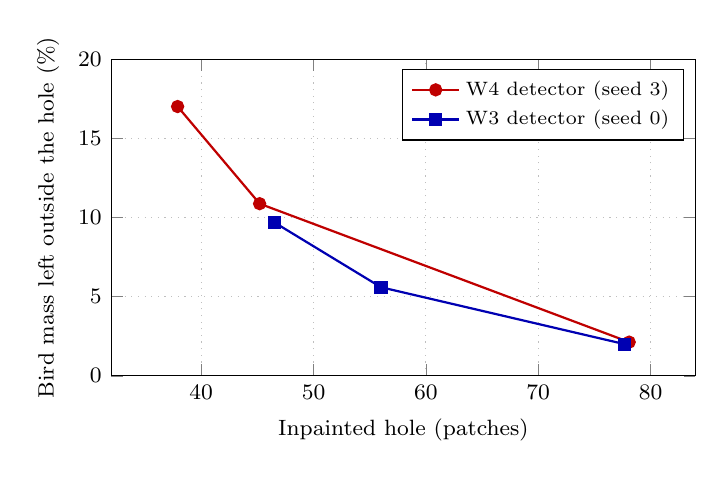
\begin{tikzpicture}
\begin{axis}[width=9cm,height=5.6cm,xlabel={Inpainted hole (patches)},ylabel={Bird mass left outside the hole (\%)},
 xmin=32,xmax=84,ymin=0,ymax=20,grid=major,grid style={dotted,gray!50},legend style={font=\scriptsize,at={(0.98,0.97)},anchor=north east},
 tick label style={font=\footnotesize},label style={font=\footnotesize}]
\addplot[mark=*,thick,red!75!black] coordinates {(37.9,17.02)(45.2,10.88)(78.1,2.13)};
\addlegendentry{W4 detector (seed 3)}
\addplot[mark=square*,thick,blue!70!black] coordinates {(46.5,9.7)(56.0,5.6)(77.7,2.0)};
\addlegendentry{W3 detector (seed 0)}
\end{axis}
\end{tikzpicture}
\end{document}
